\documentclass[11pt]{article}
\usepackage[utf8]{inputenc}
\usepackage[T1]{fontenc}
\usepackage{graphicx}
\usepackage[export]{adjustbox}
\graphicspath{ {./images/} }

\begin{document}
\section*{Reading}
Private Equity Funds as Intermediaries

PE funds serve as financial intermediaries by facilitating investment in PE. There are several motivations to using PE funds as intermediaries.

\section*{Private Equity Fund Intermediation and Risk}
Basically, PE funds step into the funding process when traditional lenders are not willing or able to provide funding. For example, banks may be unwilling to lend to an entrepreneur or be involved in LBOs because of the substantial risks that are involved. In the case of lending to an entrepreneur, the product or the intellectual property is not well understood, and of course the firm has no track record that the bank could use to evaluate its riskiness. Also, some of these lenders (e.g., banks) are not willing or allowed to take equity positions in these firms. This means they cannot fully participate in the significant upsides that PE investments could provide. These significant upside returns can justify the risks PE investors are willing to take by investing in new and untested companies or by taking significant credit and leverage risk and investing in poorly performing firms. PE investors take advantage of the inefficiencies in financial markets while satisfying the needs of these borrowers.

PE funds are generally organized as limited partnerships designed to provide limited liability to the investors. Limited liability is the protection of investors from losses that exceed their investment. LPs are not responsible for liabilities beyond the total loss of their commitment, even if the partnership has further losses and unmet liabilities due to the use of leverage or from lawsuits. To have limited liability, a partner must be a limited partner and must not take an active role in the partnership's management. The general partner does not have limited liability and takes an active role in the management of the partnership.

\section*{Private Equity Fund Intermediation and Efficient Incentives}
Another reason for the existence of PE firms is the presence of certain economic inefficiencies in the traditional corporate structure. In some cases, management may not be given proper incentives to maximize the value to the shareholders of a corporation. PE seeks to address this problem by tightly aligning the interests of managers and shareholders to achieve increased efficiency and higher return to shareholders.

\section*{Private Equity Funds Serve the Following Five Primary Functions}
PE funds may be viewed as providing five primary functions:

\begin{enumerate}
  \item Pooling investors' capital for investing in private companies.

  \item Screening, evaluating, and selecting potential companies with expected high-return opportunities.

  \item Financing companies to develop new products and technologies, foster their growth and development, make acquisitions, or allow for a buyout or a buy-in by experienced managers.

  \item Controlling, coaching, and monitoring portfolio companies. By dedicating personnel from the PE fund, the private equity firm can have more control, influence, and value creation of the portfolio company.

  \item Sourcing exit opportunities for portfolio companies.

\end{enumerate}

\section*{Forms of Private Equity Fund Intermediation}
There are different routes for investing in PE (see the PE Funds Investment Program exhibit). Few institutional investors have the experience, the incentive structures, and the access that would allow them to invest directly in nonpublic companies, so most investors seek intermediation through funds. For institutions, the most relevant approaches to investing in PE are through fund-of-funds specialists as intermediaries or through similarly structured dedicated in-house PE investment programs that invest directly in funds. Other routes are via publicly quoted PE vehicles or through a dedicated account managed by a PE specialist.\\
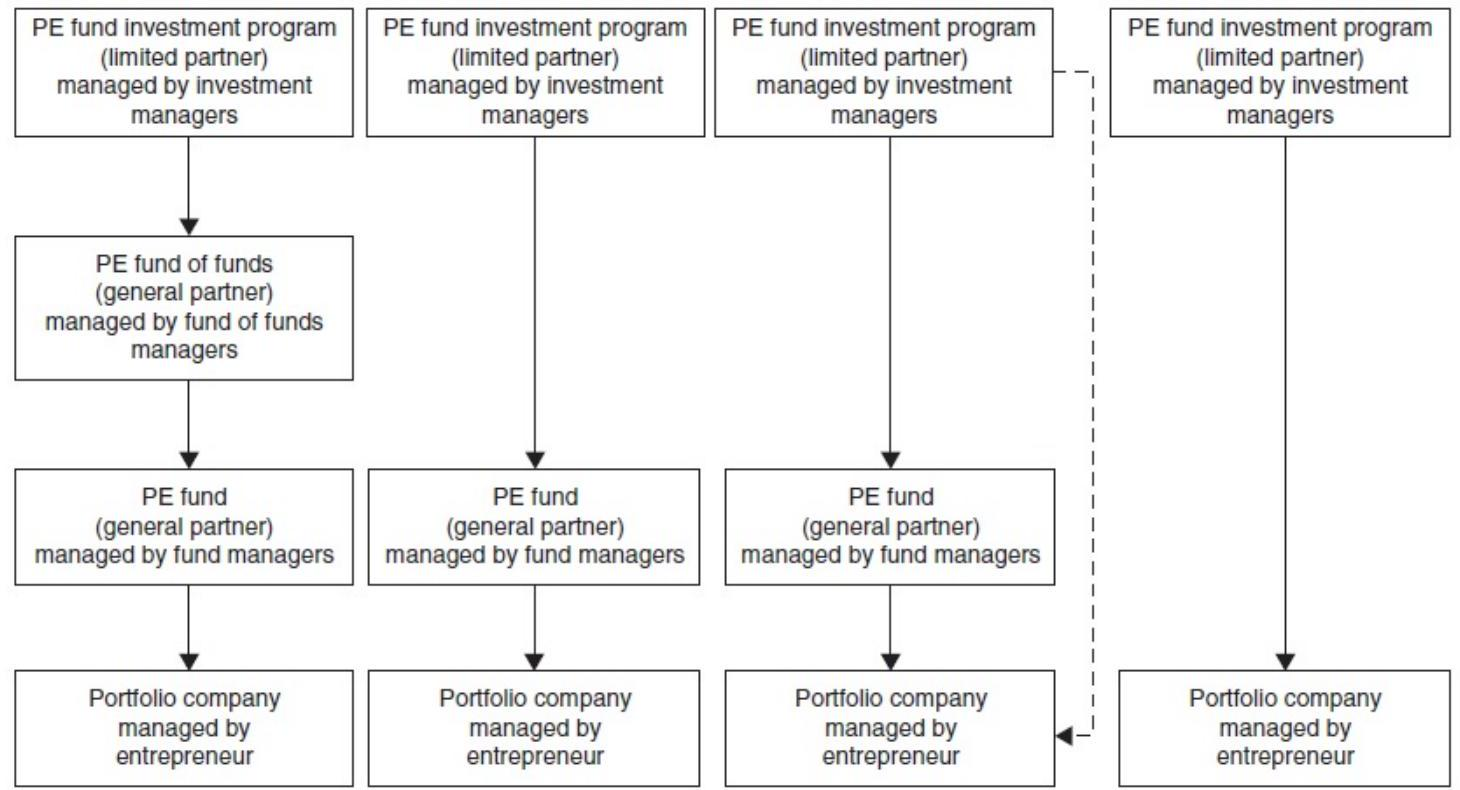
\includegraphics[max width=\textwidth, center]{2024_04_10_9afab3e78f4ed9e425bag-2}

\section*{PE Funds Investment Program}
Reading the PE Funds Investment Program exhibit above from left to right, the various programs are defined as follows:

In a fund of funds structure, an institutional PE investor buys LP units of a PE fund of funds, which in turn purchases LP units of a PE fund, which, in turn, invests in portfolio companies.

In the second column, an institutional PE investor buys LP units directly in a PE fund that invests in portfolio companies.

In the third column, a PE fund adds a co-investment to the process in the second column. The co-investment leg is where the PE fund has an additional investment in a certain portfolio company, typically at preferential management and performance fee terms. Co-investment involves investors being invited by GPs to make direct investments in portfolio companies, as is discussed in detail in the second level of the CAIA program.

Finally, the fourth column depicts direct investment by the institutional PE investor who eschews PE fund structures altogether and makes investments straight into a portfolio company (without intermediation), similar to a co-investment but without the input of a PE fund manager.

\section*{The Life Cycle of a Limited Partnership}
A limited partnership is a long-term investment. The typical term of a PE limited partnership locks up investors' capital for a minimum of 10 years. A fundraising cycle begins anew each time GPs need to raise capital for another fund. Typically, limited partnership agreements do not allow follow-on funds by the same manager before the end of the initial fund's investment period or until a large part of the initial fund has been invested.

During this long investment period, a limited partnership normally goes through five stages of development.

The fundraising stage: The first stage of a fund is the fundraising stage, in which the firm raises capital from outside investors. Capital is committed, not collected. This is an important distinction. Investors sign a legal agreement (typically a subscription) that legally binds them to make cash investments in the fund up to a specified amount. This is the committed, but not yet drawn, capital. The firm or general partner also posts committed capital. Fundraising normally takes six months to a year. However, the more successful funds can raise the funds in just a few months.

Commitments (capital pledges by investors in funds) are drawn down as needed, or just in time, to make investments or to pay costs, expenses, or management fees. Because funds do not typically retain large pools of uninvested capital, their GPs make capital calls (or drawdowns) once they have identified a company in which to invest. Therefore, the main part of the drawdown gets invested immediately.

Sourcing investments: The second stage is sourcing investments, the process of locating possible investments (i.e., generating deal flow), reading business plans, performing intense due diligence on start-up companies, and determining the attractiveness of each start-up company. This period begins the moment the fund is closed to investors and normally takes up the first three to five years of the venture fund's existence to complete. As the general partner, the manager has full operating authority to manage the fund, subject to restrictions placed in the covenants of the fund's documents. During the first two stages, no profits are generated by the fund. In fact, quite the reverse happens: The fund generates losses because the manager continues to draw annual management fees based on the total committed capital. These fees generate a loss until the manager begins to extract value from the investments of the fund at a later stage.

Investing stage: Stage three is investment of capital. During this stage, the fund manager determines how much capital to commit to each start-up company, at what level of financing, and in what form of investment (convertible preferred shares, convertible debentures, etc.). At this stage, the fund manager also makes capital calls to the investors in the fund to draw the committed capital of the LPs. Note that no cash inflow is generated yet; the fund is still in a deficit.

Generally, the year in which the fund first draws down capital from investors for the purpose of investing in a company is called the vintage year; some data providers use the year that the fund commences operations as the vintage year.

A substantial portion, though typically not all, of the committed capital is drawn down during the investment period, typically the first three to five years, during which new opportunities are identified. After that, during the divestment period, only the existing portfolio companies with the highest potential are further supported, with some follow-on funding provided to extract the maximum value through exits. The manager's efforts during this time are concentrated on realizing or selling investments.

It might surprise many investors to learn that they should expect the accounting value of their investment in a fund to drop over the first three to five years. This is because the organizational expenses of the partnership are deducted immediately. In addition, management fees are charged on committed capital by the fund's general partner. Further, those investments that fail quickly are posted as losses, while investments that are showing excellent potential are not posted as profits (if they have not already been sold). All of this means that investors must be braced for a loss on their investments for the first three to five years of a fund's life. Truly, limited partnership is for the long-term investor.

Operations and management: Stage four, which includes operation and management of the portfolio of companies, begins after all the funds have been invested, and lasts almost to the end of the term of the fund. During this time, the manager works with the portfolio companies in which the fund has invested. The manager may improve each portfolio company's management team, establish distribution channels for the new product, refine the prototype product to generate the greatest sales, and generally position the start-up company for an eventual public offering or sale to a strategic buyer. During this period, the fund manager begins to generate profits for the fund. These profits initially offset the previously collected management fees and other expenses until a positive cumulative profit is established for the fund.

Windup and liquidation: The last stage of the fund is its windup and liquidation. At this point, all committed capital has been invested, and the fund is now in the harvesting stage. Each of the fund's portfolio companies faces possible outcomes: being sold to a strategic or a financial buyer, being brought to the public markets in an initial public offering (IPO), or being liquidated through a bankruptcy liquidation process. Profits are distributed to the LPs, and the general partner/fund manager now collects the incentive/profit-sharing fees.

When realizations (sales of portfolio companies) are made, or when interest payments, dividends, or recapitalizations are received, they are distributed to investors as soon as is feasible. Under this scenario, the fund liquidates as the underlying investments are realized. However, these returns come mostly in the second half of the fund's lifetime. However, some funds have a reinvestment provision, normally subject to a cap amount, wherein the proceeds of realizations within the investment period or a similar time frame may be reinvested in new opportunities and not distributed to investors.

Distributions to investors can also take the form of securities of a portfolio company, known as in-kind distributions, provided that these securities are publicly tradable or distributed when the fund gets liquidated. Legal documentation may also allow for some reinvestment of realizations.

The exhibit below shows the typical Fund Standard J-Curve. It plots the interim IRRs and the lifetime IRR of a typical fund. The J-curve is the classic illustration of the early losses and later likely profitability of a fund. The central return measurement for a fund is the IRR method detailed in the session Quantitative Foundations. The shape of the J-curve is determined by two factors, namely, Capital Calls and Distributions. In addition, the life cycle of a fund can be divided into three periods:

\begin{itemize}
  \item The first is the investment period, which is typically the first two to three years of the fund. During the investment period, capital can be called for management fees, as well as for investment into portfolio companies. There is typically no Distribution from portfolio companies as the GP is just starting to put the cash to work. The fund IRR is initially negative, as the management exceed the distributed profits from exits of portfolio company investments.
  \item The second is the value creation period, which is typically from year three to year five of the fund. The GP still makes Capital Calls from LPs for management fees, but most of the capital has already been deployed. Instead, the underlying portfolio companies may provide Distributions allowing the GP to distribute cashflow to LPs.
  \item The third phase is the harvest period, which is typically from year four onwards. The GP may exit their investments when the conditions are right. When the investments are realized, the cash is returned to LPs. As the size and number of exits increases, the fund IRR starts to turn positive.
\end{itemize}

\begin{center}
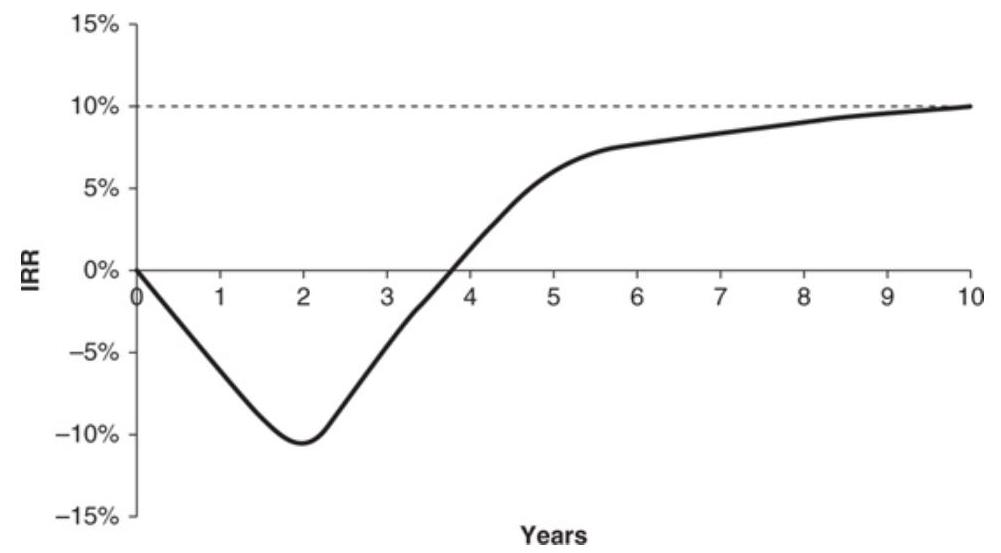
\includegraphics[max width=\textwidth]{2024_04_10_9afab3e78f4ed9e425bag-4}
\end{center}

Fund Standard J-Curve

While the typical fund J-curve shows a hockey stick shape, as seen in the exhibit above, the use of subscription lines may flip the shape of the J-curve. When the fund uses a subscription line for investments and expenses, no capital is called from the LPs. However, when an investment is marked upward, this will result in a very high interim IRR since there is very little cash outflow and a significant Net Asset Value increase. The interim IRR averages down as capital is called from LPs. This results in the IRR profile looking like an inverted hockey stick.

Other J-curves can also be observed in funds: the cash flow J-curve and the net asset value (NAV) J-curve. The NAV of a fund is calculated by adding the value of all the investments held in the fund and dividing by the number of outstanding shares of the fund. The NAV J-curve is a representation of the evolution of the NAV of a fund versus the net paid in (NPI), which first decreases during the early years of the fund's existence and then improves in its later years.

The cash flow J-curve is a representation of the evolution of the net accumulated cash flows from the investors to the fund, which are negative during the early years of existence before making a U-turn and becoming positive in the later years of the fund's life. The net accumulated cash flows may last for several years before turning positive. This is explained by the fact that in standard fund structures, commitments are drawn down as needed, or just in time, and when realizations are made after having successfully developed these newly founded companies, they are distributed as soon as is practical.

\section*{Undrawn Capital Commitments}
Undrawn capital commitments are a liability of the associated investors. While they are often viewed as irrelevant to the investment's value (since the calls of capital commitments are used to fund investments that belong to the partnership), undrawn commitments caused serious problems for some LPs during the global financial crises and led to the coining of the terms commitment risk or funding risk. Commitment risk describes the situation in which an LP may become a defaulting investor when they do not have sufficient liquidity to pay the capital calls of newly committed funds. Commitment risk is discussed in the next section.

\section*{Four Substantial Risks of Private Equity}
PE has specific characteristics that are not shared by other asset classes. The most substantial risks in this asset class are market risk, liquidity risk, commitment or funding risk, and realization risk (EVCA 2013):

\begin{enumerate}
  \item Market risk: Market risk is economic uncertainty with regard to the value of an asset, in this case an illiquid asset. Listed assets are valued using market prices. Illiquid assets are often valued using an analysis of the present value of the estimated future cash flows from that asset. Market prices and professional valuations often signal different levels of market risk.

  \item Liquidity risk: LPs can sell their stakes in PE partnerships to fund their outstanding commitments. However, the secondary market for PE investments is relatively small and inefficient. Secondary market prices may be influenced by factors beyond the fair value of the partnership, which often means that prices are discounted. Liquidity risk plays a far less important role for public equities.

  \item Commitment or funding risk: The unpredictable timing of cash flows over the life of a fund poses funding risk for the limited partner. Fund managers call most or all of the committed capital over the investment period of the fund. LPs then have to meet their commitments within a fixed short-notice period. Because commitments are contractually binding, limited partners who cannot meet their obligations are forced to default on payments and lose a substantial portion of or even their entire share in the partnership.

  \item Realization risk: PE investors face the long-term risk of not recovering the value of their invested capital at realization. This long-term capital risk can be affected by a number of factors, namely (1) the ability of managers to create value and extract cash from exiting the companies, (2) the level of equity markets\\
and IPO activity at the time of exit, and (3) risks specific to the company.

\end{enumerate}

\section*{Strategies to Mitigate Risks of Private Equity}
\begin{enumerate}
  \item Market risk mitigation: Market risk can produce unrealized or "paper" losses and these short-term impairments may result in realized losses if a PE fund does not have adequate time or capital to allow for a correction. An LP can mitigate market risk by building a diversified portfolio of PE funds by region, sector, currency, and vintage years, thereby limiting the impact of a disruption in any single or localized sector or market or market cycle.

  \item Liquidity risk mitigation: Selling an LP interest in the secondary market may take several weeks or months to complete, if it can even be accomplished. Furthermore, the value obtained may potentially be at a discount to a PE fund's reported NAV for such LP interest. Ideally, LPs should have sufficient resources and exposure to other liquid assets in order to enable them to hold their LP interests until maturity, thereby effectively mitigating their liquidity risk.

  \item Funding risk mitigation: Funding risk is the risk that an LP cannot meet its capital commitment obligations. While the timing of capital calls in respect of a PE fund is variable, particularly within the PE fund's investment period, the total capital call is generally capped at the original capital commitment amount.

  \item Realization risk mitigation: Although it is common for an individual portfolio company in a PE fund to be completely written off, the impact of individual losses can be substantially reduced through the creation of a diversified portfolio of PE funds with several hundred underlying companies. This benefit of diversification is driven by the statistical observation that, while a PE fund can generally only lose up to its initial investment in a portfolio company, a wellperforming investment can generate a return of several times its original cost. Ideally, LPs should build a diversified portfolio, so that well-performing investments can more than offset the losses of poor-performing investments, skewing the aggregate portfolio performance to positive returns.

\end{enumerate}

\end{document}